% Lifting Autogyro Unit --- Cross-Section v3 (Final)
% Compile: pdflatex assembly_v3.tex
\documentclass{article}
\usepackage[paperwidth=22cm,paperheight=16cm,margin=0.2cm]{geometry}
\usepackage{amsmath,amssymb,tikz}
\usetikzlibrary{arrows.meta,calc,patterns,decorations.pathreplacing,positioning}

\begin{document}
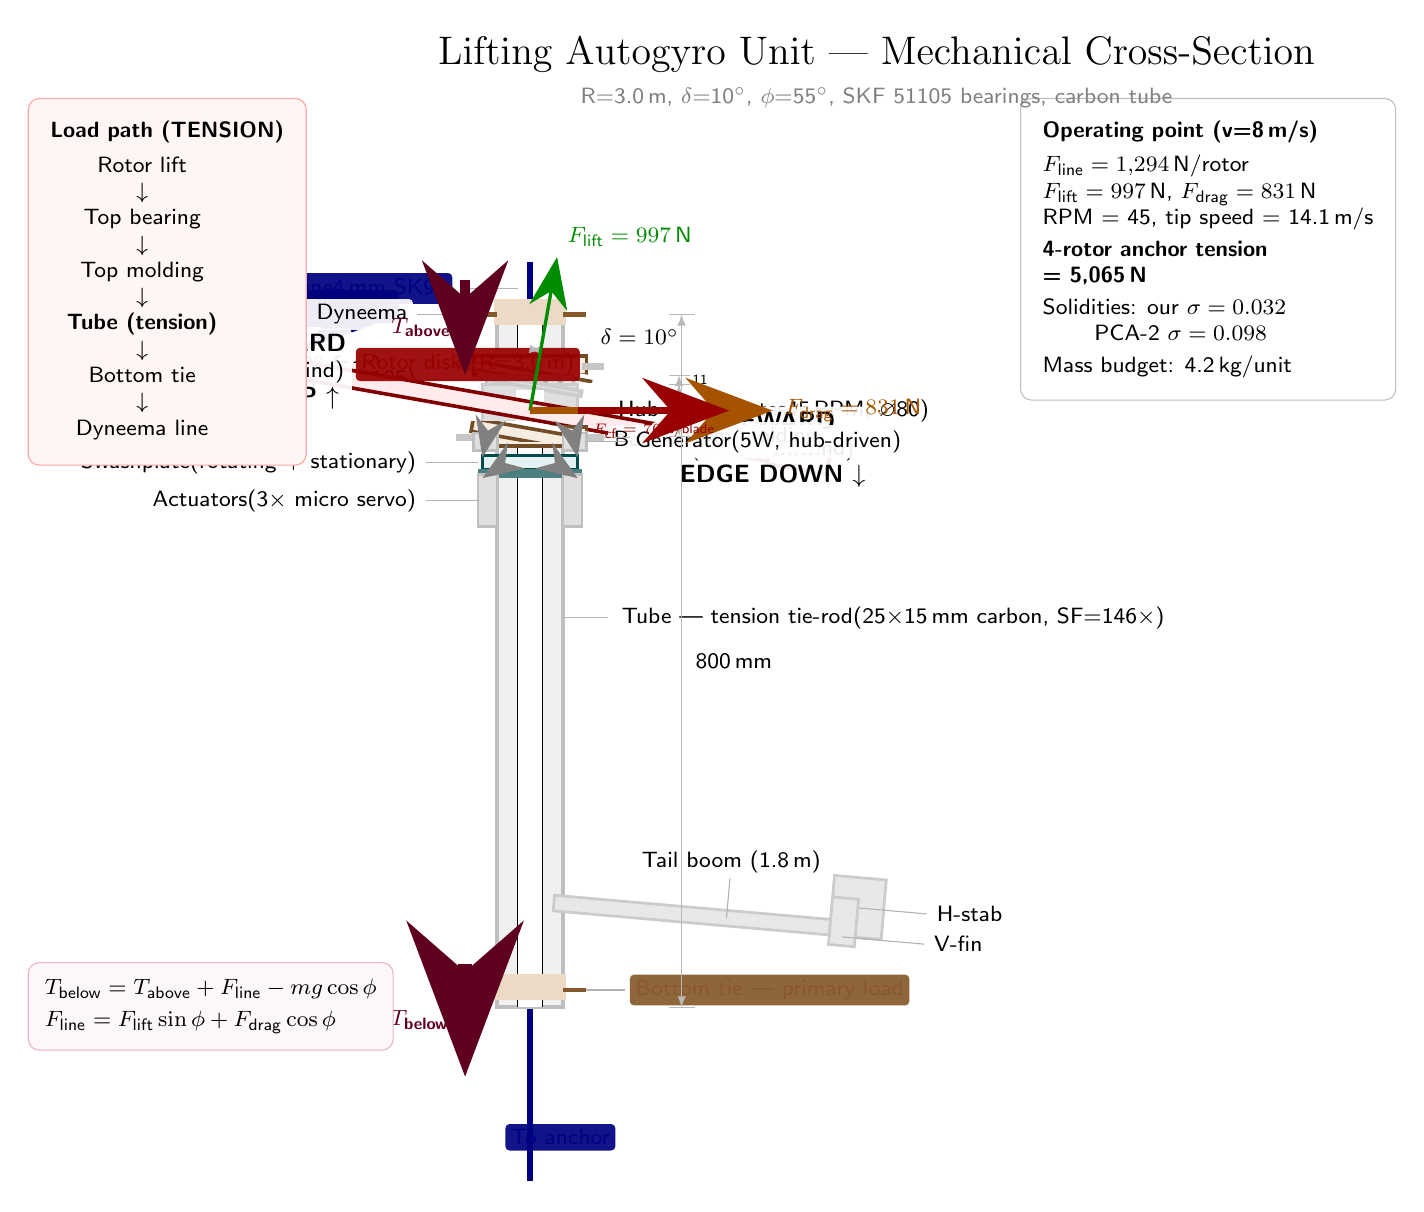
\begin{tikzpicture}[
    scale=1.1,
    dyneema/.style={draw=blue!50!black, line width=2.0pt},
    tube/.style={draw=gray!50, fill=gray!12, line width=1.5pt},
    molding/.style={draw=brown!60!black, fill=brown!15, line width=1.3pt},
    bearing/.style={draw=gray!50, fill=gray!20, line width=1.0pt},
    hub/.style={draw=gray!40, fill=gray!25, line width=1.3pt},
    rotor/.style={draw=red!50!black, fill=red!8, line width=1.3pt},
    blade/.style={draw=red!45!black, fill=red!6, line width=1.3pt},
    actuator/.style={draw=gray!50, fill=gray!25, line width=1.0pt},
    swash/.style={draw=teal!60!black, fill=teal!10, line width=1.0pt},
    empennage/.style={draw=gray!40, fill=gray!18, line width=1.0pt},
    generator/.style={draw=gray!50, fill=gray!25, line width=1.0pt},
    force/.style={-{Stealth[scale=2.2]}, line width=2.5pt},
    forcecomp/.style={-{Stealth[scale=1.5]}, line width=1.5pt, densely dashed},
    dimline/.style={latex-latex, thin, draw=gray!55},
    dimext/.style={thin, draw=gray!55},
    annot/.style={font=\footnotesize\sffamily, fill=white, fill opacity=0.93,
                  text opacity=1, inner sep=2pt, rounded corners=1.5pt},
    annotW/.style={font=\footnotesize\sffamily, fill=white, fill opacity=0.93,
                   text=white, inner sep=2pt, rounded corners=1.5pt},
    label/.style={font=\small\sffamily\bfseries},
]

% Coordinates: +Z=up (tube axial). Wind +X=right. -X edge = windward = UP.
\def\tilt{10}
\def\tubetop{8.0}\def\tubebot{0}
\def\toptieZ{8.0}\def\topmoldZ{7.3}\def\topbearZ{7.3}
\def\hubtopZ{7.19}\def\rotorZ{6.89}\def\hubbotZ{6.59}
\def\botbearZ{6.59}\def\botmoldZ{6.48}
\def\genZ{6.53}\def\swashZ{6.15}\def\actZ{5.55}
\def\empZ{1.2}\def\bottieZ{0.2}
\def\moldH{0.22}\def\bearingH{0.11}\def\hubH{0.6}

% ============================================================
% DYNEMA LINE + TUBE + WIND
% ============================================================
% Dyneema through center
\draw[dyneema] (0, \tubebot-2.0) -- (0, \tubetop+0.6);

% Wind arrow --- blows toward +X (right)
\draw[force, blue!45!black, line width=2.0pt]
    (-3.8, \rotorZ+1.0) -- (-1.8, \rotorZ+1.0);
\node[annot, blue!45!black] at (-2.8, \rotorZ+1.2) {Wind $v_\infty=8$\,m/s $\to$};

% Tube
\fill[tube] (-0.38, \tubebot) rectangle (0.38, \tubetop);
\draw[tube] (-0.38, \tubebot) -- (-0.38, \tubetop);
\draw[tube] (0.38, \tubebot) -- (0.38, \tubetop);
\fill[white] (-0.14, \tubebot) rectangle (0.14, \tubetop);
\draw[thin] (-0.14, \tubebot) -- (-0.14, \tubetop);
\draw[thin] (0.14, \tubebot) -- (0.14, \tubetop);

% Tube label
\draw[thin, gray!60] (0.38, 4.5) -- (0.9, 4.5);
\node[annot, right=0.1cm] at (0.9, 4.5) {Tube --- tension tie-rod\\(25$\times$15\,mm carbon, SF=146$\times$)};

% Dyneema label
\draw[thin, gray!60] (-0.14, \tubetop+0.3) -- (-0.8, \tubetop+0.3);
\node[annot, blue!50!black, left=0.1cm] at (-0.8, \tubetop+0.3) {Dyneema line\\4\,mm SK99};

% ============================================================
% TOP TIE
% ============================================================
\fill[brown!30] (-0.42, \toptieZ-0.12) rectangle (0.42, \toptieZ+0.18);
\draw[brown!70!black, line width=1.5pt] (-0.65, \toptieZ) -- (-0.38, \toptieZ);
\draw[brown!70!black, line width=1.5pt] (0.38, \toptieZ) -- (0.65, \toptieZ);
\draw[thin, gray!60] (-0.65, \toptieZ) -- (-1.3, \toptieZ);
\node[annot, left=0.05cm] at (-1.3, \toptieZ) {Top tie $\rightarrow$ Dyneema};

% ============================================================
% TOP MOLDING --- angled underside at $\delta$ (CW tilt: windward edge UP)
% ============================================================
\fill[molding] (-0.65, \topmoldZ) rectangle (0.65, \topmoldZ+\moldH);
\begin{scope}
    \clip (-1.0, \topmoldZ-0.08) rectangle (1.0, \topmoldZ+0.15);
    \fill[white, rotate around={-\tilt:(0,\topmoldZ)}]
        (-1.0, \topmoldZ-0.08) rectangle (1.0, \topmoldZ+0.12);
    \fill[molding, rotate around={-\tilt:(0,\topmoldZ)}]
        (-0.7, \topmoldZ-0.05) rectangle (0.7, \topmoldZ+0.05);
\end{scope}
\fill[gray!45] (0.6, \topmoldZ+0.06) rectangle (0.85, \topmoldZ+0.14);
\fill[gray!45] (-0.6, \topmoldZ+0.06) rectangle (-0.85, \topmoldZ+0.14);
\draw[thin, gray!60] (-0.85, \topmoldZ+0.1) -- (-1.6, \topmoldZ+0.1);
\node[annot, left=0.05cm] at (-1.6, \topmoldZ+0.1) {Top molding (10$^\circ$ face)};

% ============================================================
% TOP BEARING --- SKF 51105
% ============================================================
\fill[bearing] (-0.5, \topbearZ-\bearingH) rectangle (0.5, \topbearZ);
\foreach \x in {-0.35,-0.18,0,0.18,0.35} {
    \fill[gray!60] (\x, \topbearZ-\bearingH/2) circle (0.04);
}
\draw[thin, gray!60] (-0.5, \topbearZ-\bearingH/2) -- (-1.2, \topbearZ-\bearingH/2);
\node[annot, left=0.05cm] at (-1.2, \topbearZ-\bearingH/2) {Top bearing (SKF 51105)};

% ============================================================
% ROTOR HUB
% ============================================================
\fill[hub] (-0.55, \hubbotZ) rectangle (0.55, \hubtopZ);
\fill[hub, rotate around={-\tilt:(0,\hubtopZ)}]
    (-0.6, \hubtopZ-0.03) rectangle (0.6, \hubtopZ+0.03);
\fill[hub, rotate around={-\tilt:(0,\hubbotZ)}]
    (-0.6, \hubbotZ-0.03) rectangle (0.6, \hubbotZ+0.03);
\fill[white] (-0.16, \hubbotZ+0.06) rectangle (0.16, \hubtopZ-0.06);
\draw[thin, gray!60] (0.55, \rotorZ) -- (0.9, \rotorZ);
\node[annot, right=0.05cm] at (0.9, \rotorZ) {Hub (autorotates\\45\,RPM, $\varnothing$80)};

% ============================================================
% ROTOR DISK + BLADES --- CW tilt: -X (windward) edge UP
% ============================================================
\begin{scope}[rotate around={-\tilt:(0,\rotorZ)}]
    % Disk
    \fill[rotor] (-2.8, \rotorZ-0.1) rectangle (2.8, \rotorZ+0.1);
    % Disk label
    \node[annot, red!60!black] at (-0.8, \rotorZ+0.4) {Rotor disk (R=3.0\,m)};
    % Blades
    \fill[blade] (-3.5, \rotorZ-0.13) rectangle (-2.8, \rotorZ+0.13);
    \fill[blade] (2.8, \rotorZ-0.13) rectangle (3.5, \rotorZ+0.13);
\end{scope}

% Edge labels --- clarify which side is UP
\node[annot, align=center] at (-3.0, \rotorZ+0.45)
    {\small\bfseries WINDWARD\\\footnotesize(-X, into wind)\\\small\bfseries EDGE UP $\uparrow$};
\node[annot, align=center] at (2.8, \rotorZ-0.45)
    {\small\bfseries LEEWARD\\\footnotesize(+X, downwind)\\\small\bfseries EDGE DOWN $\downarrow$};

% Blade label
\draw[thin, gray!60] (-3.8, \rotorZ) -- (-4.3, \rotorZ);
\node[annot, left=0.05cm] at (-4.3, \rotorZ) {Blade (2$\times$)};

% Tilt angle with dimension arc
\draw[dimline] (0, \rotorZ+0.7) arc[start angle=90, end angle={90-\tilt}, radius=0.7cm];
\node[annot, right=0.05cm] at (0.7, \rotorZ+0.85) {$\delta=10^\circ$};

% ============================================================
% BOTTOM BEARING
% ============================================================
\fill[bearing] (-0.5, \botbearZ-\bearingH) rectangle (0.5, \botbearZ);
\foreach \x in {-0.35,-0.18,0,0.18,0.35} {
    \fill[gray!60] (\x, \botbearZ-\bearingH/2) circle (0.04);
}
\draw[thin, gray!60] (0.5, \botbearZ-\bearingH/2) -- (0.85, \botbearZ-\bearingH/2);
\node[annot, right=0.05cm] at (0.85, \botbearZ-\bearingH/2) {Bottom bearing};

% ============================================================
% BOTTOM MOLDING
% ============================================================
\fill[molding] (-0.65, \botmoldZ) rectangle (0.65, \botmoldZ+\moldH);
\begin{scope}
    \clip (-1.0, \botmoldZ+0.05) rectangle (1.0, \botmoldZ+0.28);
    \fill[white, rotate around={-\tilt:(0,\botmoldZ)}]
        (-1.0, \botmoldZ+0.12) rectangle (1.0, \botmoldZ+0.28);
    \fill[molding, rotate around={-\tilt:(0,\botmoldZ)}]
        (-0.7, \botmoldZ+0.05) rectangle (0.7, \botmoldZ+0.2);
\end{scope}
\fill[gray!45] (0.6, \botmoldZ+0.06) rectangle (0.85, \botmoldZ+0.14);
\fill[gray!45] (-0.6, \botmoldZ+0.06) rectangle (-0.85, \botmoldZ+0.14);
\draw[thin, gray!60] (0.85, \botmoldZ+0.1) -- (1.35, \botmoldZ+0.1);
\node[annot, right=0.05cm] at (1.35, \botmoldZ+0.1) {Bottom molding};

% ============================================================
% GENERATOR
% ============================================================
\fill[generator] (0.38, \genZ-0.1) rectangle (0.65, \genZ+0.1);
\fill[generator] (-0.38, \genZ-0.1) rectangle (-0.65, \genZ+0.1);
\draw[thin, gray!60] (0.65, \genZ) -- (1.1, \genZ);
\node[annot, right=0.05cm] at (1.1, \genZ) {Generator\\(5W, hub-driven)};

% ============================================================
% SWASHPLATE + ACTUATORS
% ============================================================
\fill[swash] (-0.55, \swashZ+0.06) rectangle (0.55, \swashZ+0.22);
\fill[teal!40!gray] (-0.6, \swashZ-0.04) rectangle (0.6, \swashZ+0.06);
\draw[thin, gray!60] (-0.6, \swashZ+0.14) -- (-1.2, \swashZ+0.14);
\node[annot, left=0.05cm] at (-1.2, \swashZ+0.14) {Swashplate\\(rotating + stationary)};

% Scissor links
\draw[forcecomp, gray] (0.5, \hubbotZ) -- (0.55, \swashZ+0.2);
\draw[forcecomp, gray] (-0.5, \hubbotZ) -- (-0.55, \swashZ+0.2);

\fill[actuator] (0.38, \actZ) rectangle (0.6, \actZ+0.6);
\fill[actuator] (-0.38, \actZ) rectangle (-0.6, \actZ+0.6);
\draw[forcecomp, gray] (0.49, \actZ+0.6) -- (0.55, \swashZ-0.04);
\draw[forcecomp, gray] (-0.49, \actZ+0.6) -- (-0.55, \swashZ-0.04);
\draw[thin, gray!60] (-0.6, \actZ+0.3) -- (-1.2, \actZ+0.3);
\node[annot, left=0.05cm] at (-1.2, \actZ+0.3) {Actuators\\(3$\times$ micro servo)};

% ============================================================
% EMPENNAGE
% ============================================================
\begin{scope}[shift={(0.38, \empZ)}, rotate around={-5:(0,\empZ)}]
    \fill[empennage] (0, -0.09) rectangle (3.8, 0.09);
    \draw[thin, gray!60] (2.0, 0.0) -- (2.0, 0.5);
    \node[annot] at (2.0, 0.65) {Tail boom (1.8\,m)};
    \fill[empennage] (3.2, -0.09) rectangle (3.8, 0.6);
    \draw[thin, gray!60] (3.5, 0.25) -- (4.3, 0.25);
    \node[annot, right=0.05cm] at (4.3, 0.25) {H-stab};
    \fill[empennage] (3.2, 0.35) rectangle (3.5, -0.2);
    \draw[thin, gray!60] (3.35, -0.1) -- (4.3, -0.1);
    \node[annot, right=0.05cm] at (4.3, -0.1) {V-fin};
\end{scope}

% ============================================================
% BOTTOM TIE --- primary load path
% ============================================================
\fill[brown!30] (-0.42, \bottieZ-0.12) rectangle (0.42, \bottieZ+0.18);
\draw[brown!70!black, line width=1.5pt] (-0.65, \bottieZ) -- (-0.38, \bottieZ);
\draw[brown!70!black, line width=1.5pt] (0.38, \bottieZ) -- (0.65, \bottieZ);
\draw[thin, gray!60] (0.65, \bottieZ) -- (1.1, \bottieZ);
\node[annot, brown!70!black, right=0.05cm] at (1.1, \bottieZ) {Bottom tie --- primary load};

% Anchor extension
\node[annot, blue!50!black] at (0.35, \tubebot-1.5) {To anchor};

% ============================================================
% DIMENSIONS with extension lines
% ============================================================
% Tube length
\draw[dimext] (1.6, \tubebot) -- (1.9, \tubebot);
\draw[dimext] (1.6, \tubetop) -- (1.9, \tubetop);
\draw[dimline] (1.75, \tubebot) -- (1.75, \tubetop);
\node[annot, right=0.1cm] at (1.75, 4.0) {800\,mm};

% Bearing height
\draw[dimext] (1.6, \topbearZ) -- (1.85, \topbearZ);
\draw[dimext] (1.6, \topbearZ-\bearingH) -- (1.85, \topbearZ-\bearingH);
\draw[dimline] (1.72, \topbearZ-\bearingH) -- (1.72, \topbearZ);
\node[font=\tiny\sffamily, right=0.05cm] at (1.72, \topbearZ-\bearingH/2) {11};

% Hub height
\draw[dimext] (1.6, \hubtopZ) -- (1.85, \hubtopZ);
\draw[dimext] (1.6, \hubbotZ) -- (1.85, \hubbotZ);
\draw[dimline] (1.72, \hubbotZ) -- (1.72, \hubtopZ);
\node[font=\tiny\sffamily, right=0.05cm] at (1.72, \rotorZ) {60};

% ============================================================
% FORCE ARROWS --- cleanly separated
% ============================================================

% T_above --- left side
\draw[force, purple!50!black, line width=3.5pt]
    (-0.75, \tubetop+0.4) -- (-0.75, \topmoldZ)
    node[midway, left, font=\footnotesize\sffamily\bfseries, purple!50!black] {$T_\text{above}$};

% T_below --- left side, thicker
\draw[force, purple!50!black, line width=5pt]
    (-0.75, \tubebot+0.5) -- (-0.75, \tubebot-0.8)
    node[midway, left, font=\footnotesize\sffamily\bfseries, purple!50!black] {$T_\text{below}$};

% F_lift --- green, from disk center perp wind
\draw[force, green!55!black, very thick]
    (0, \rotorZ) -- ++({1.8*sin(\tilt)}, {1.8*cos(\tilt)})
    node[above right, font=\footnotesize\sffamily, green!55!black] {$F_\text{lift}=997$\,N};

% F_drag --- orange, parallel wind
\draw[force, orange!65!black]
    (0, \rotorZ) -- ++(2.8, 0)
    node[right, font=\footnotesize\sffamily, orange!65!black] {$F_\text{drag}=831$\,N};

% F_centrifugal --- red, radially OUTWARD
\draw[force, red!60!black, line width=2.5pt]
    (0.55, \rotorZ) -- (2.3, \rotorZ)
    node[midway, below, font=\tiny\sffamily, red!60!black] {$F_\text{cf}=70$\,N/blade};

% ============================================================
% INFO PANELS (positioned in margins, clear of drawing)
% ============================================================

% Load path --- top left
\node[draw=red!35, fill=red!4, rounded corners=4pt, inner sep=8pt,
      anchor=north west, font=\footnotesize\sffamily, align=left]
    at (-5.8, 10.5) {
    \textbf{Load path (TENSION)}\\[3pt]
    \begin{tabular}{c}
    Rotor lift\\
    $\downarrow$\\
    Top bearing\\
    $\downarrow$\\
    Top molding\\
    $\downarrow$\\
    \textbf{Tube (tension)}\\
    $\downarrow$\\
    Bottom tie\\
    $\downarrow$\\
    Dyneema line
    \end{tabular}
};

% Operating point --- top right
\node[draw=black!25, fill=white, rounded corners=4pt, inner sep=8pt,
      anchor=north east, font=\footnotesize\sffamily, align=left]
    at (10.0, 10.5) {
    \textbf{Operating point (v=8\,m/s)}\\[3pt]
    $F_\text{line} = 1,\!294$\,N/rotor\\
    $F_\text{lift}=997$\,N, $F_\text{drag}=831$\,N\\
    RPM = 45, tip speed = 14.1\,m/s\\[2pt]
    \textbf{4-rotor anchor tension}\\
    \textbf{= 5,065\,N}\\[2pt]
    Solidities: our $\sigma=0.032$\\
    \hspace{2.2em}PCA-2 $\sigma=0.098$\\[2pt]
    Mass budget: 4.2\,kg/unit
};

% Tension equation --- bottom left
\node[draw=purple!30, fill=purple!3, rounded corners=4pt, inner sep=6pt,
      anchor=south west, font=\footnotesize\sffamily, align=left]
    at (-5.8, -0.5) {
    $T_\text{below} = T_\text{above} + F_\text{line} - mg\cos\phi$\\[2pt]
    $F_\text{line} = F_\text{lift}\sin\phi + F_\text{drag}\cos\phi$
};

% ============================================================
% TITLE
% ============================================================
\node[label, font=\Large] at (4.0, 11.0)
    {Lifting Autogyro Unit --- Mechanical Cross-Section};

\node[font=\footnotesize\sffamily, gray] at (4.0, 10.5)
    {R=3.0\,m, $\delta$=10$^\circ$, $\phi$=55$^\circ$, SKF 51105 bearings, carbon tube};

\end{tikzpicture}
\end{document}
